\documentclass{standalone}
\usepackage{tikz}
\usetikzlibrary{patterns, positioning}

\begin{document}
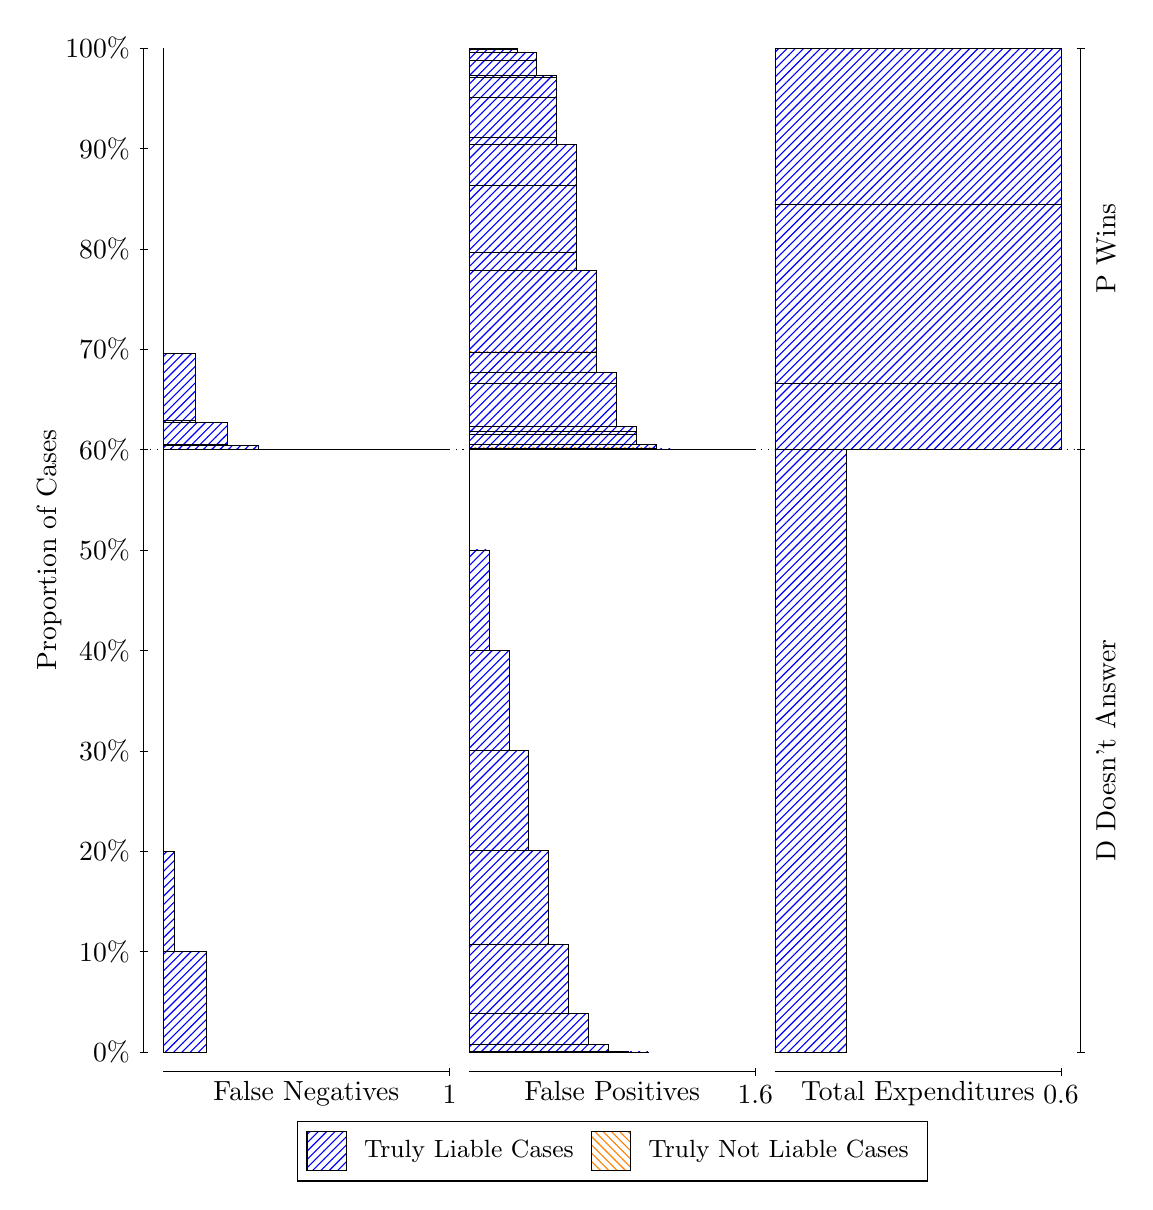
\begin{tikzpicture}
\draw[black, very thin] (1.5,1.75) -- (1.5,14.5);
\node[rotate=90, anchor=center] at (0.3, 8.125) {Proportion of Cases};
\draw[black, very thin] (1.45,1.75) -- (1.55,1.75);
\node[anchor=east] at (1.45, 1.75) {0\%};
\draw[black, very thin] (1.45,3.025) -- (1.55,3.025);
\node[anchor=east] at (1.45, 3.025) {10\%};
\draw[black, very thin] (1.45,4.3) -- (1.55,4.3);
\node[anchor=east] at (1.45, 4.3) {20\%};
\draw[black, very thin] (1.45,5.575) -- (1.55,5.575);
\node[anchor=east] at (1.45, 5.575) {30\%};
\draw[black, very thin] (1.45,6.85) -- (1.55,6.85);
\node[anchor=east] at (1.45, 6.85) {40\%};
\draw[black, very thin] (1.45,8.125) -- (1.55,8.125);
\node[anchor=east] at (1.45, 8.125) {50\%};
\draw[black, very thin] (1.45,9.4) -- (1.55,9.4);
\node[anchor=east] at (1.45, 9.4) {60\%};
\draw[black, very thin] (1.45,10.675) -- (1.55,10.675);
\node[anchor=east] at (1.45, 10.675) {70\%};
\draw[black, very thin] (1.45,11.95) -- (1.55,11.95);
\node[anchor=east] at (1.45, 11.95) {80\%};
\draw[black, very thin] (1.45,13.225) -- (1.55,13.225);
\node[anchor=east] at (1.45, 13.225) {90\%};
\draw[black, very thin] (1.45,14.5) -- (1.55,14.5);
\node[anchor=east] at (1.45, 14.5) {100\%};

\draw[black, very thin] (13.4,1.75) -- (13.4,14.5);
\draw[black, very thin] (13.35,1.75) -- (13.45,1.75);
\node[anchor=west] at (13.35, 1.75) {};
\draw[black, very thin] (13.35,9.4014) -- (13.45,9.4014);
\node[anchor=west] at (13.35, 9.4014) {};
\draw[black, very thin] (13.35,14.5) -- (13.45,14.5);
\node[anchor=west] at (13.35, 14.5) {};

\draw[black, very thin, pattern color=blue, pattern=north east lines] (1.75,1.75) rectangle (2.295,3.025);
\draw[black, very thin, pattern color=blue, pattern=north east lines] (1.75,3.025) rectangle (1.8913,4.3);
\draw[black, very thin, pattern color=orange, pattern=north west lines] (1.75,4.3) rectangle (1.75,4.3);
\draw[black, very thin, pattern color=blue, pattern=north east lines] (1.75,4.3) rectangle (1.75,9.4014);
\draw[black, very thin, pattern color=blue, pattern=north east lines] (1.75,9.4014) rectangle (5.3833,9.4014);
\draw[black, very thin, pattern color=blue, pattern=north east lines] (1.75,9.4014) rectangle (4.9796,9.4014);
\draw[black, very thin, pattern color=blue, pattern=north east lines] (1.75,9.4014) rectangle (4.5759,9.4014);
\draw[black, very thin, pattern color=blue, pattern=north east lines] (1.75,9.4014) rectangle (4.5759,9.4014);
\draw[black, very thin, pattern color=blue, pattern=north east lines] (1.75,9.4014) rectangle (4.1722,9.4014);
\draw[black, very thin, pattern color=blue, pattern=north east lines] (1.75,9.4014) rectangle (4.1722,9.4014);
\draw[black, very thin, pattern color=blue, pattern=north east lines] (1.75,9.4014) rectangle (3.7685,9.4015);
\draw[black, very thin, pattern color=blue, pattern=north east lines] (1.75,9.4015) rectangle (3.3648,9.4022);
\draw[black, very thin, pattern color=blue, pattern=north east lines] (1.75,9.4022) rectangle (3.3648,9.4056);
\draw[black, very thin, pattern color=blue, pattern=north east lines] (1.75,9.4056) rectangle (2.9611,9.4088);
\draw[black, very thin, pattern color=blue, pattern=north east lines] (1.75,9.4088) rectangle (2.9611,9.4579);
\draw[black, very thin, pattern color=blue, pattern=north east lines] (1.75,9.4579) rectangle (2.9611,9.4579);
\draw[black, very thin, pattern color=blue, pattern=north east lines] (1.75,9.4579) rectangle (2.5574,9.4674);
\draw[black, very thin, pattern color=blue, pattern=north east lines] (1.75,9.4674) rectangle (2.5574,9.7491);
\draw[black, very thin, pattern color=blue, pattern=north east lines] (1.75,9.7491) rectangle (2.1537,9.7672);
\draw[black, very thin, pattern color=blue, pattern=north east lines] (1.75,9.7672) rectangle (2.1537,10.618);
\draw[black, very thin, pattern color=blue, pattern=north east lines] (1.75,10.618) rectangle (2.1537,10.62);
\draw[black, very thin, pattern color=orange, pattern=north west lines] (1.75,10.62) rectangle (1.75,10.62);
\draw[black, very thin, pattern color=blue, pattern=north east lines] (1.75,10.62) rectangle (1.75,14.5);
\draw[black, very thin, pattern color=orange, pattern=north west lines] (5.6333,1.75) rectangle (7.9042,1.75);
\draw[black, very thin, pattern color=blue, pattern=north east lines] (5.6333,1.75) rectangle (7.9042,1.7504);
\draw[black, very thin, pattern color=blue, pattern=north east lines] (5.6333,1.7504) rectangle (7.6519,1.7589);
\draw[black, very thin, pattern color=blue, pattern=north east lines] (5.6333,1.7589) rectangle (7.3995,1.8446);
\draw[black, very thin, pattern color=blue, pattern=north east lines] (5.6333,1.8446) rectangle (7.1472,2.2381);
\draw[black, very thin, pattern color=blue, pattern=north east lines] (5.6333,2.2381) rectangle (6.8949,3.1197);
\draw[black, very thin, pattern color=blue, pattern=north east lines] (5.6333,3.1197) rectangle (6.6426,4.3095);
\draw[black, very thin, pattern color=blue, pattern=north east lines] (5.6333,4.3095) rectangle (6.3903,5.5766);
\draw[black, very thin, pattern color=blue, pattern=north east lines] (5.6333,5.5766) rectangle (6.138,6.8513);
\draw[black, very thin, pattern color=blue, pattern=north east lines] (5.6333,6.8513) rectangle (5.8856,8.1263);
\draw[black, very thin, pattern color=blue, pattern=north east lines] (5.6333,8.1263) rectangle (5.6333,9.4014);
\draw[black, very thin, pattern color=orange, pattern=north west lines] (5.6333,9.4014) rectangle (9.2667,9.4014);
\draw[black, very thin, pattern color=blue, pattern=north east lines] (5.6333,9.4014) rectangle (9.2667,9.4014);
\draw[black, very thin, pattern color=orange, pattern=north west lines] (5.6333,9.4014) rectangle (9.0144,9.4014);
\draw[black, very thin, pattern color=blue, pattern=north east lines] (5.6333,9.4014) rectangle (9.0144,9.4014);
\draw[black, very thin, pattern color=orange, pattern=north west lines] (5.6333,9.4014) rectangle (8.762,9.4014);
\draw[black, very thin, pattern color=blue, pattern=north east lines] (5.6333,9.4014) rectangle (8.762,9.4014);
\draw[black, very thin, pattern color=blue, pattern=north east lines] (5.6333,9.4014) rectangle (8.5097,9.4015);
\draw[black, very thin, pattern color=orange, pattern=north west lines] (5.6333,9.4015) rectangle (8.5097,9.4015);
\draw[black, very thin, pattern color=blue, pattern=north east lines] (5.6333,9.4015) rectangle (8.5097,9.402);
\draw[black, very thin, pattern color=blue, pattern=north east lines] (5.6333,9.402) rectangle (8.2574,9.4036);
\draw[black, very thin, pattern color=orange, pattern=north west lines] (5.6333,9.4036) rectangle (8.2574,9.4036);
\draw[black, very thin, pattern color=blue, pattern=north east lines] (5.6333,9.4036) rectangle (8.2574,9.4095);
\draw[black, very thin, pattern color=blue, pattern=north east lines] (5.6333,9.4095) rectangle (8.0051,9.4211);
\draw[black, very thin, pattern color=orange, pattern=north west lines] (5.6333,9.4211) rectangle (8.0051,9.4211);
\draw[black, very thin, pattern color=blue, pattern=north east lines] (5.6333,9.4211) rectangle (8.0051,9.4615);
\draw[black, very thin, pattern color=blue, pattern=north east lines] (5.6333,9.4615) rectangle (7.7528,9.4618);
\draw[black, very thin, pattern color=orange, pattern=north west lines] (5.6333,9.4618) rectangle (7.7528,9.4618);
\draw[black, very thin, pattern color=blue, pattern=north east lines] (5.6333,9.4618) rectangle (7.7528,9.5906);
\draw[black, very thin, pattern color=blue, pattern=north east lines] (5.6333,9.5906) rectangle (7.7528,9.638);
\draw[black, very thin, pattern color=blue, pattern=north east lines] (5.6333,9.638) rectangle (7.7528,9.6952);
\draw[black, very thin, pattern color=blue, pattern=north east lines] (5.6333,9.6952) rectangle (7.5005,9.6961);
\draw[black, very thin, pattern color=orange, pattern=north west lines] (5.6333,9.6961) rectangle (7.5005,9.6961);
\draw[black, very thin, pattern color=blue, pattern=north east lines] (5.6333,9.6961) rectangle (7.5005,10.239);
\draw[black, very thin, pattern color=blue, pattern=north east lines] (5.6333,10.239) rectangle (7.5005,10.377);
\draw[black, very thin, pattern color=blue, pattern=north east lines] (5.6333,10.377) rectangle (7.2481,10.377);
\draw[black, very thin, pattern color=blue, pattern=north east lines] (5.6333,10.377) rectangle (7.2481,10.642);
\draw[black, very thin, pattern color=orange, pattern=north west lines] (5.6333,10.642) rectangle (7.2481,10.642);
\draw[black, very thin, pattern color=blue, pattern=north east lines] (5.6333,10.642) rectangle (7.2481,11.674);
\draw[black, very thin, pattern color=blue, pattern=north east lines] (5.6333,11.674) rectangle (6.9958,11.907);
\draw[black, very thin, pattern color=orange, pattern=north west lines] (5.6333,11.907) rectangle (6.9958,11.907);
\draw[black, very thin, pattern color=blue, pattern=north east lines] (5.6333,11.907) rectangle (6.9958,12.763);
\draw[black, very thin, pattern color=blue, pattern=north east lines] (5.6333,12.763) rectangle (6.9958,13.281);
\draw[black, very thin, pattern color=blue, pattern=north east lines] (5.6333,13.281) rectangle (6.7435,13.364);
\draw[black, very thin, pattern color=blue, pattern=north east lines] (5.6333,13.364) rectangle (6.7435,13.869);
\draw[black, very thin, pattern color=blue, pattern=north east lines] (5.6333,13.869) rectangle (6.7435,14.134);
\draw[black, very thin, pattern color=blue, pattern=north east lines] (5.6333,14.134) rectangle (6.7435,14.152);
\draw[black, very thin, pattern color=blue, pattern=north east lines] (5.6333,14.152) rectangle (6.4912,14.344);
\draw[black, very thin, pattern color=blue, pattern=north east lines] (5.6333,14.344) rectangle (6.4912,14.443);
\draw[black, very thin, pattern color=blue, pattern=north east lines] (5.6333,14.443) rectangle (6.4912,14.443);
\draw[black, very thin, pattern color=blue, pattern=north east lines] (5.6333,14.443) rectangle (6.2389,14.444);
\draw[black, very thin, pattern color=blue, pattern=north east lines] (5.6333,14.444) rectangle (6.2389,14.478);
\draw[black, very thin, pattern color=blue, pattern=north east lines] (5.6333,14.478) rectangle (6.2389,14.496);
\draw[black, very thin, pattern color=blue, pattern=north east lines] (5.6333,14.496) rectangle (6.2389,14.496);
\draw[black, very thin, pattern color=blue, pattern=north east lines] (5.6333,14.496) rectangle (5.9866,14.499);
\draw[black, very thin, pattern color=blue, pattern=north east lines] (5.6333,14.499) rectangle (5.9866,14.5);
\draw[black, very thin, pattern color=blue, pattern=north east lines] (5.6333,14.5) rectangle (5.7343,14.5);
\draw[black, very thin, pattern color=blue, pattern=north east lines] (5.6333,14.5) rectangle (5.7343,14.5);
\draw[black, very thin, pattern color=blue, pattern=north east lines] (5.6333,14.5) rectangle (5.7343,14.5);
\draw[black, very thin, pattern color=blue, pattern=north east lines] (5.6333,14.5) rectangle (5.6333,14.5);
\draw[black, very thin, pattern color=orange, pattern=north west lines] (9.5167,1.75) rectangle (10.425,1.75);
\draw[black, very thin, pattern color=blue, pattern=north east lines] (9.5167,1.75) rectangle (10.425,9.4014);
\draw[black, very thin, pattern color=orange, pattern=north west lines] (9.5167,9.4014) rectangle (13.15,9.4014);
\draw[black, very thin, pattern color=blue, pattern=north east lines] (9.5167,9.4014) rectangle (13.15,10.244);
\draw[black, very thin, pattern color=orange, pattern=north west lines] (9.5167,10.244) rectangle (13.15,10.244);
\draw[black, very thin, pattern color=blue, pattern=north east lines] (9.5167,10.244) rectangle (13.15,12.513);
\draw[black, very thin, pattern color=orange, pattern=north west lines] (9.5167,12.513) rectangle (13.15,12.513);
\draw[black, very thin, pattern color=blue, pattern=north east lines] (9.5167,12.513) rectangle (13.15,14.5);
\draw[black, dotted] (1.5,9.4014) -- (13.4,9.4014);
\draw[black, very thin] (1.75,1.5) -- (5.3833,1.5);
\node[anchor=north] at (3.5667, 1.5) {False Negatives};
\draw[black, very thin] (5.3833,1.45) -- (5.3833,1.55);
\node[anchor=north] at (5.3833, 1.45) {1};

\draw[black, very thin] (5.6333,1.5) -- (9.2667,1.5);
\node[anchor=north] at (7.45, 1.5) {False Positives};
\draw[black, very thin] (9.2667,1.45) -- (9.2667,1.55);
\node[anchor=north] at (9.2667, 1.45) {1.6};

\draw[black, very thin] (9.5167,1.5) -- (13.15,1.5);
\node[anchor=north] at (11.333, 1.5) {Total Expenditures};
\draw[black, very thin] (13.15,1.45) -- (13.15,1.55);
\node[anchor=north] at (13.15, 1.45) {0.6};

\node[black, centered, rotate=90] at (13.72, 5.5757) {D Doesn't Answer};
\node[black, centered, rotate=90] at (13.72, 11.951) {P Wins};

\draw (7.449999999999999,1.5) node[draw=none] (baseCoordinate) {};
\begin{scope}[align=center]
        \matrix[scale=0.5, draw=black, below=0.5cm of baseCoordinate, nodes={draw}, column sep=0.1cm]{
            \node[rectangle, draw, minimum width=0.5cm, minimum height=0.5cm, pattern=north east lines, pattern color=blue] {}; &
            \node[draw=none, font=\small] (B) {Truly Liable Cases}; &
            \node[rectangle, draw, minimum width=0.5cm, minimum height=0.5cm, pattern=north west lines, pattern color=orange] {}; &
            \node[draw=none, font=\small] (B) {Truly Not Liable Cases}; \\
            };
\end{scope}

\end{tikzpicture}
\end{document}